\documentclass[border=3pt]{standalone}
% Shared preamble for the standalone figures of qurl_explained.tex.
% Build a figure from this folder:   tectonic fig_<name>.tex
% Colours: blue = full precision (FP), orange = 8-bit.
\usepackage[T1]{fontenc}
\usepackage{lmodern}
\usepackage{amsmath,amssymb}
\usepackage[dvipsnames]{xcolor}
\usepackage{tikz}
\usetikzlibrary{positioning,arrows.meta,calc,decorations.pathreplacing}
\usepackage{pgfplots}
\pgfplotsset{compat=1.17}
\colorlet{fp}{RoyalBlue}
\colorlet{qb}{BurntOrange}
\colorlet{good}{ForestGreen}
\colorlet{bad}{BrickRed}
\newcommand{\pold}{\pi_{\mathrm{old}}}
\newcommand{\thold}{\theta_{\mathrm{old}}}
\newcommand{\qthold}{\hat\theta_{\mathrm{old}}}
\tikzset{
  box/.style={draw, rounded corners=3pt, align=center, inner sep=4pt, font=\small},
  arr/.style={-{Stealth[length=2.2mm]}, thick},
  lab/.style={font=\footnotesize, align=center},
}
\pgfplotsset{
  small axes/.style={
    tick label style={font=\footnotesize}, label style={font=\footnotesize},
    title style={font=\small}, every axis plot/.append style={line join=round}},
}

\begin{document}
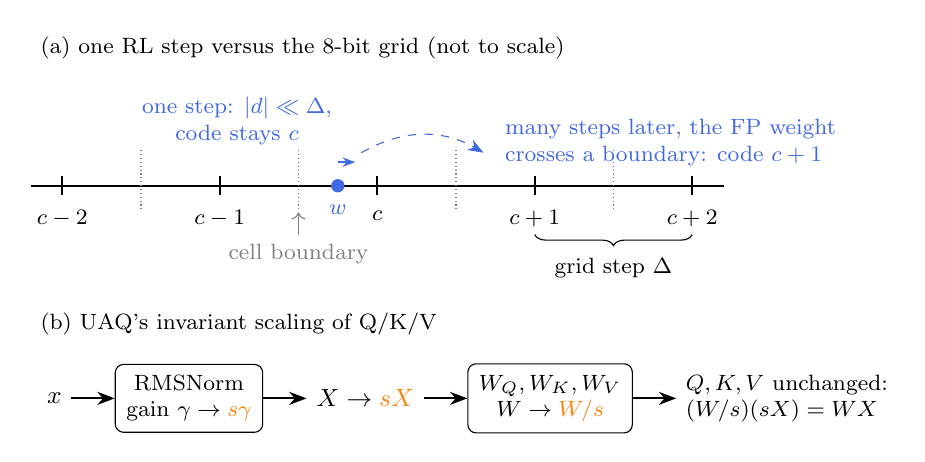
\begin{tikzpicture}[font=\small]
% (a) one step versus the grid step (not to scale)
\node[lab, anchor=west] at (-0.4,1.75) {(a) one RL step versus the 8-bit grid (not to scale)};
\draw[thick] (-0.4,0) -- (8.4,0);
\foreach \x/\l in {0/{c-2},2/{c-1},4/{c},6/{c+1},8/{c+2}} {
  \draw[thick] (\x,-0.12) -- (\x,0.12);
  \node[font=\footnotesize, below=2pt] at (\x,-0.12) {$\l$};
}
\foreach \x in {1,3,5,7} \draw[densely dotted, gray] (\x,-0.3) -- (\x,0.45);
\draw[decorate, decoration={brace, amplitude=4pt, mirror}] (6,-0.62) -- (8,-0.62) node[midway, below=5pt, font=\footnotesize] {grid step $\Delta$};
\node[lab, gray, anchor=north] at (3,-0.62) {cell boundary};
\draw[gray, ->] (3,-0.62) -- (3,-0.34);
% the weight and one step
\fill[fp] (3.5,0) circle (2.4pt);
\node[fp, font=\footnotesize, below=3pt] at (3.5,-0.02) {$w$};
\draw[-{Stealth[length=1.6mm]}, fp, thick] (3.5,0.3) -- (3.72,0.3);
\node[lab, fp, anchor=south east] at (3.55,0.4) {one step: $|d|\ll\Delta$,\\ code stays $c$};
% many steps
\draw[-{Stealth[length=2mm]}, fp, dashed] (3.8,0.42) to[out=30, in=150] (5.35,0.42);
\node[lab, fp, anchor=west, align=left] at (5.5,0.55) {many steps later, the FP weight\\ crosses a boundary: code $c+1$};
% (b) invariant scaling
\begin{scope}[yshift=-2.7cm]
\node[lab, anchor=west] at (-0.4,0.95) {(b) UAQ's invariant scaling of Q/K/V};
\node (x) at (-0.1,0) {$x$};
\node[box, right=0.55cm of x, font=\footnotesize] (norm) {RMSNorm\\ gain $\gamma\to\textcolor{qb}{s\gamma}$};
\node[right=0.55cm of norm] (X) {$X\to\textcolor{qb}{sX}$};
\node[box, right=0.55cm of X, font=\footnotesize] (qkv) {$W_Q,W_K,W_V$\\ $W\to\textcolor{qb}{W/s}$};
\node[right=0.55cm of qkv, align=left, font=\footnotesize] (out) {$Q,K,V$ unchanged:\\ $(W/s)(sX)=WX$};
\draw[arr] (x) -- (norm); \draw[arr] (norm) -- (X); \draw[arr] (X) -- (qkv); \draw[arr] (qkv) -- (out);
\end{scope}
\end{tikzpicture}
\end{document}
